\documentclass[fadttsterUserGuide_use]{subfiles}

\newpage
\begin{document}
	\section{Statistical data plotting}
	\begin{figure}[H]
  		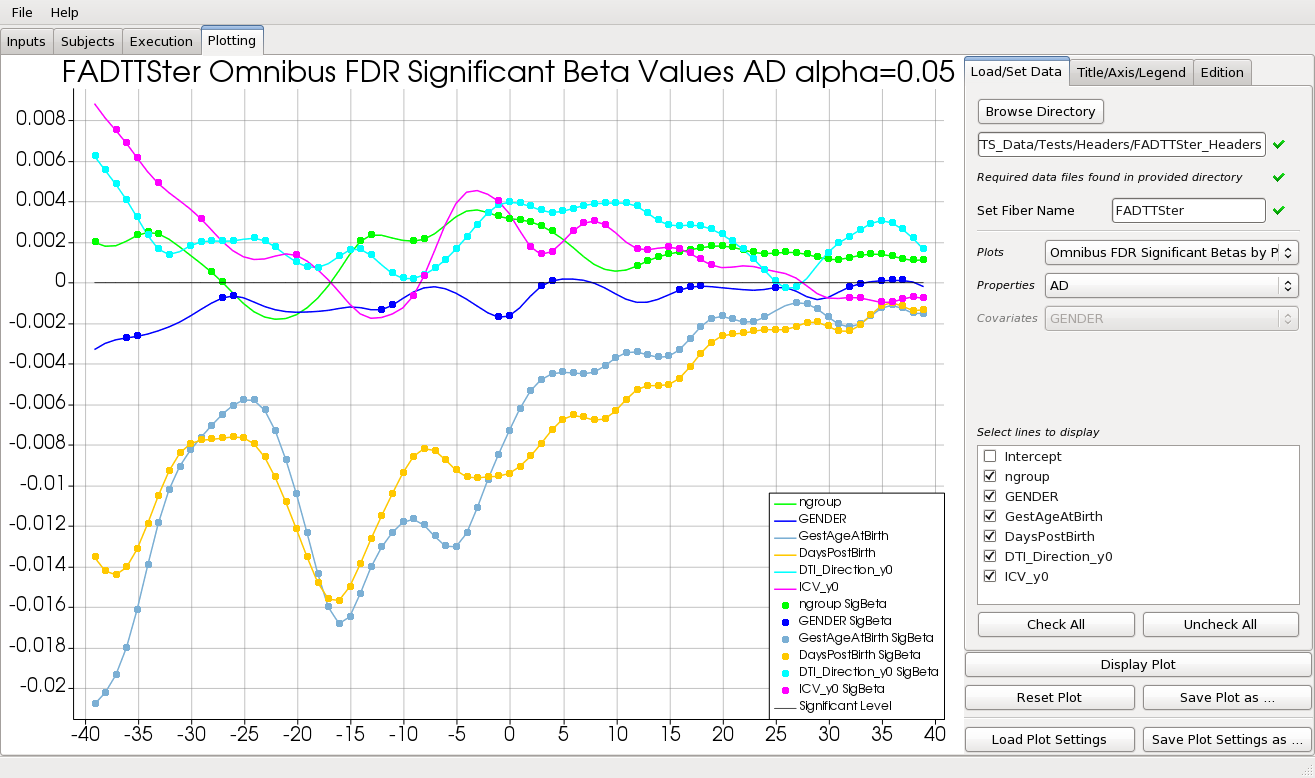
\includegraphics[width=1.36\textwidth,center]{plottingTab_filed}
  		\caption{Plotting tab}
    	\label{fig:plottingTab_filed}
	\end{figure}
	The inputs generated and the data computed by running the Matlab script in the \textit{Matlab script generation} process can be plotted within the GUI in its fourth and last tab: the Plotting Tab.
It also allows customization of the plots.	
	\vfill
	\newpage
	
	\subsection{Add plots}
	\begin{itemize}
		\item \textbf{Browsing:}
		\begin{enumerate}
			\item Click on ``Browse Directory''
			\item Browse to the folder containing the raw data files
			\item Click on ``Open''
		\end{enumerate}	
		\item \textbf{Giving an absolute path}
	\end{itemize}
	\subparagraph{\textbf{Note:}}
	\begin{itemize}
		\item[--] If the folder's name is FADTTSter\_\textit{FiberName} then \textit{FiberName} automatically extracted and set as the fiber name for the edition. Otherwise the user should set it. The fiber name can be modified at any time without any consequences.
		\item[--] Once the directory containing the statistical data is set, the plotting becomes available only if the data files found in the directory enable a plot. Otherwise, even if the folder contains some data, the plotting will remain unavailable.
	\end{itemize}
	\subsection{Display plot}
	Once the data is loaded, the user can choose to plot it. Here is how to do it:
	\begin{enumerate}
			\item Select the plot you want to display
			\begin{figure}[H]
  				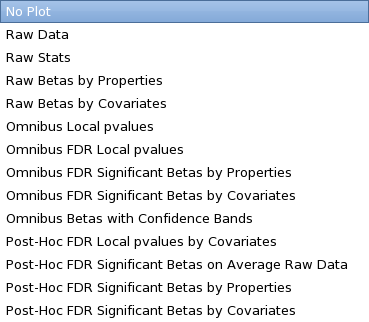
\includegraphics[width=0.54\textwidth,center]{plotsAvailable}
  				\caption{Plots available}
    			\label{fig:plotsAvailable}
			\end{figure}
			\item Select a property -- \textit{AD, RD, MD or FA} -- (only if needed)
			\item Select a covariate (only if needed)
			\item Click on ``Display Plot''
	\end{enumerate}
	\vfill
	\newpage
	
	All the plots are avaible are summarized below:
	\begin{itemize}
		\item \textbf{Raw Data}\\
		Property\textrightarrow mandatory\\
		Covariate\textrightarrow optional
		\begin{figure}[H]
  			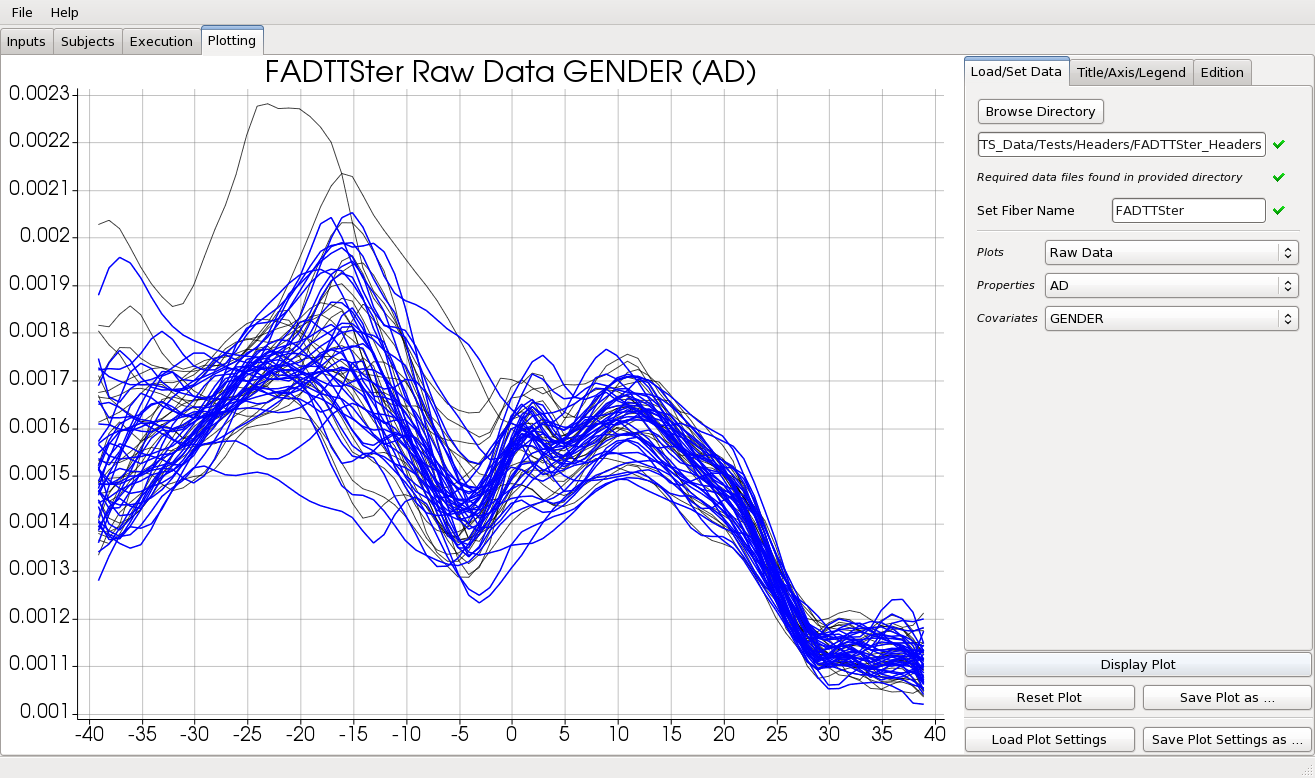
\includegraphics[width=0.9\textwidth,center]{RawData}
  			\caption{Plotting raw data}
    		\label{fig:RawData}
		\end{figure}
		\item \textbf{Raw Stats}\\
		Property\textrightarrow mandatory\\
		Covariate\textrightarrow optional
		\begin{figure}[H]
  			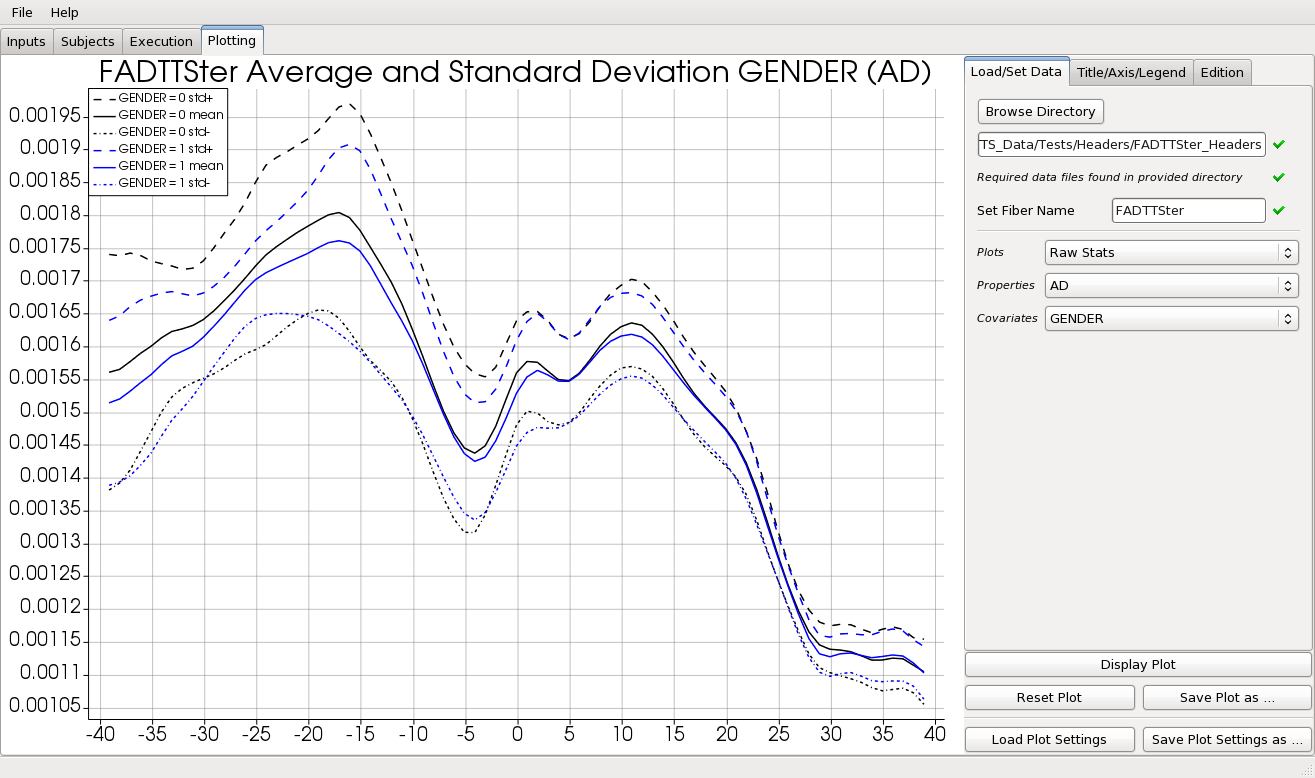
\includegraphics[width=0.9\textwidth,center]{RawStats}
  			\caption{Plotting raw stats}
    		\label{fig:RawStats}
		\end{figure}
		\vfill
		\newpage
		
		\item \textbf{Raw Betas by Properties}\\
		Property\textrightarrow mandatory\\
		Covariate\textrightarrow not required
		\begin{figure}[H]
  			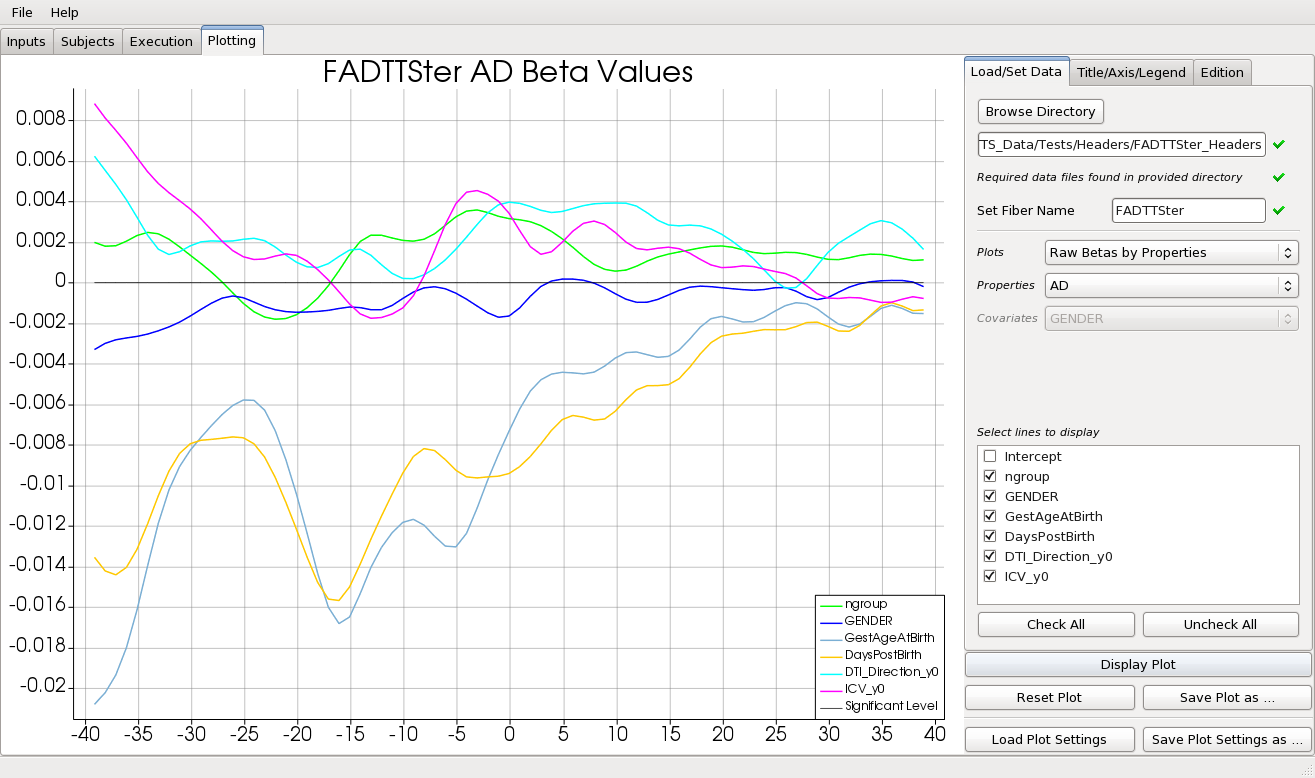
\includegraphics[width=0.95\textwidth,center]{RawBetasProp}
  			\caption{Plotting raw betas by properties}
    		\label{fig:RawBetasProp}
		\end{figure}		
		\item \textbf{Raw Betas by Covariates}\\
		Property\textrightarrow not required\\
		Covariate\textrightarrow mandatory
		\begin{figure}[H]
  			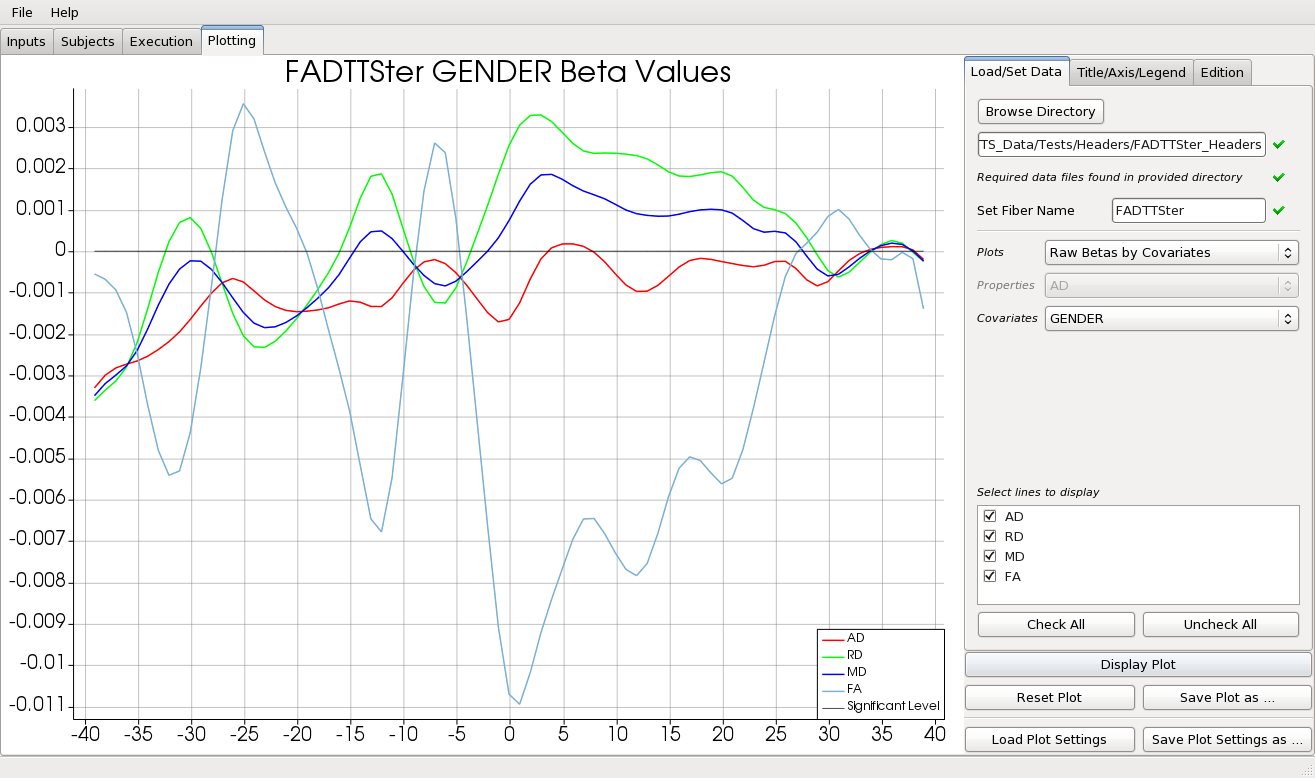
\includegraphics[width=0.95\textwidth,center]{RawBetasCov}
  			\caption{Plotting raw betas by covariates}
    		\label{fig:RawBetasCov}
		\end{figure}
		\vfill
		\newpage
		
		\item \textbf{Omnibus Local pvalues}\\
		Property\textrightarrow not required\\
		Covariate\textrightarrow not required
		\begin{figure}[H]
  			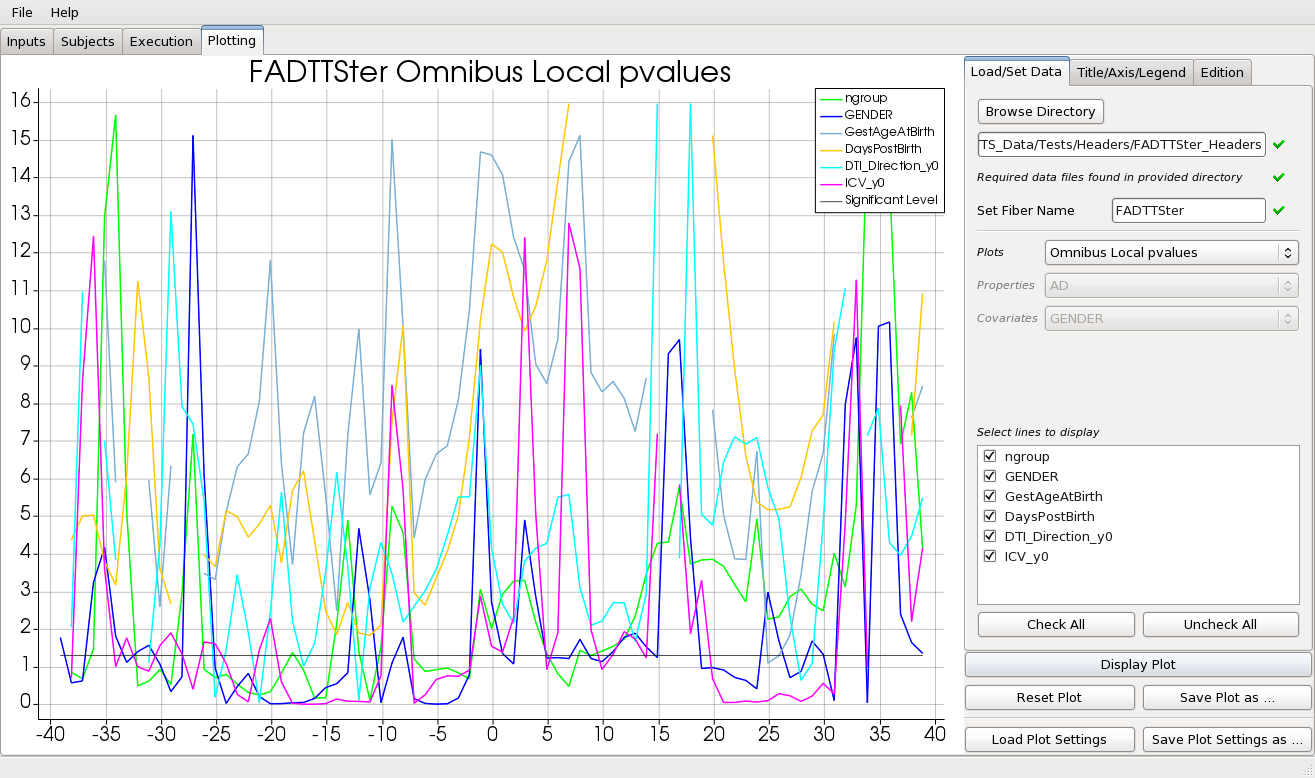
\includegraphics[width=0.95\textwidth,center]{omnibusLp}
  			\caption{Plotting omnibus local pvalues}
    		\label{fig:omnibusLp}
		\end{figure}
		\item \textbf{Omnibus FDR Local pvalues}\\
		Property\textrightarrow not required\\
		Covariate\textrightarrow not required
		\begin{figure}[H]
  			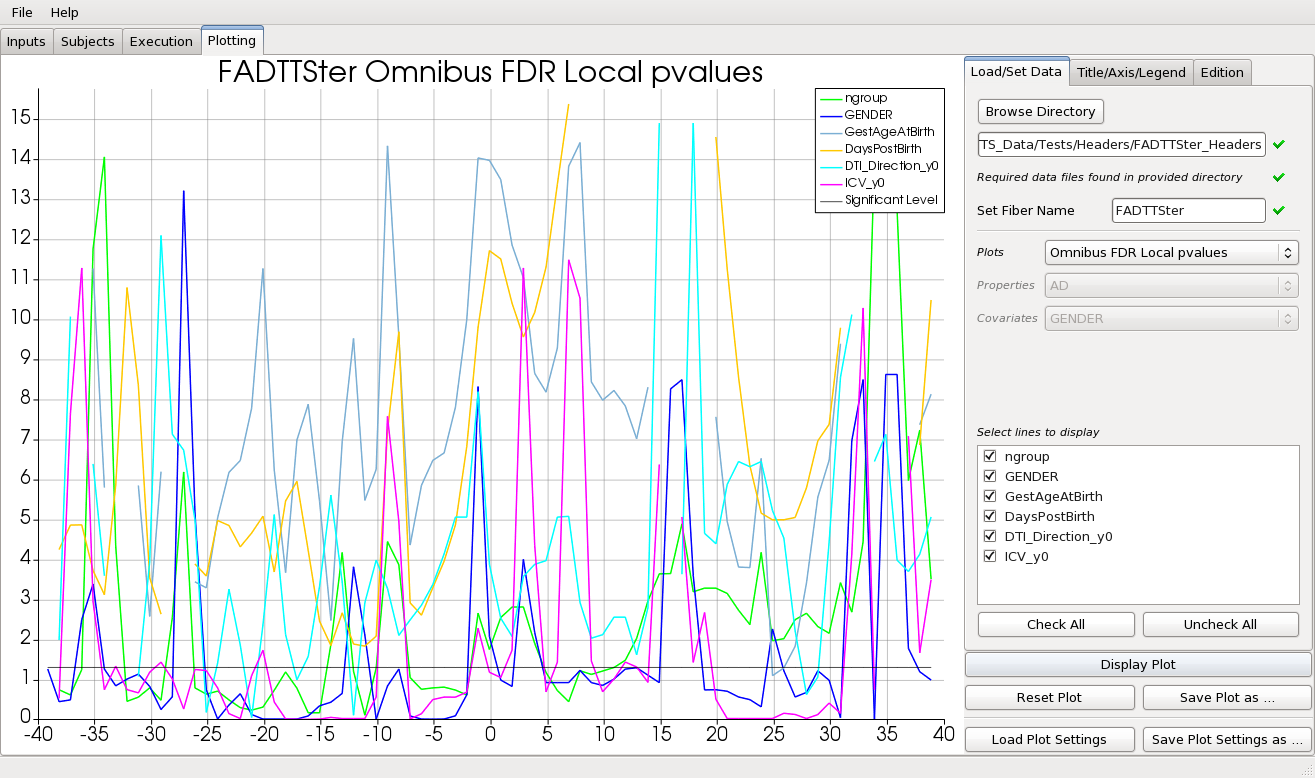
\includegraphics[width=0.95\textwidth,center]{omnibusFDRLp}
  			\caption{Plotting omnibus FDR local pvalues}
    		\label{fig:omnibusFDRLp}
		\end{figure}
		\vfill
		\newpage
		
		\item \textbf{Omnibus FDR Significant Betas by Properties}\\
		Property\textrightarrow mandatory\\
		Covariate\textrightarrow not required
		\begin{figure}[H]
  			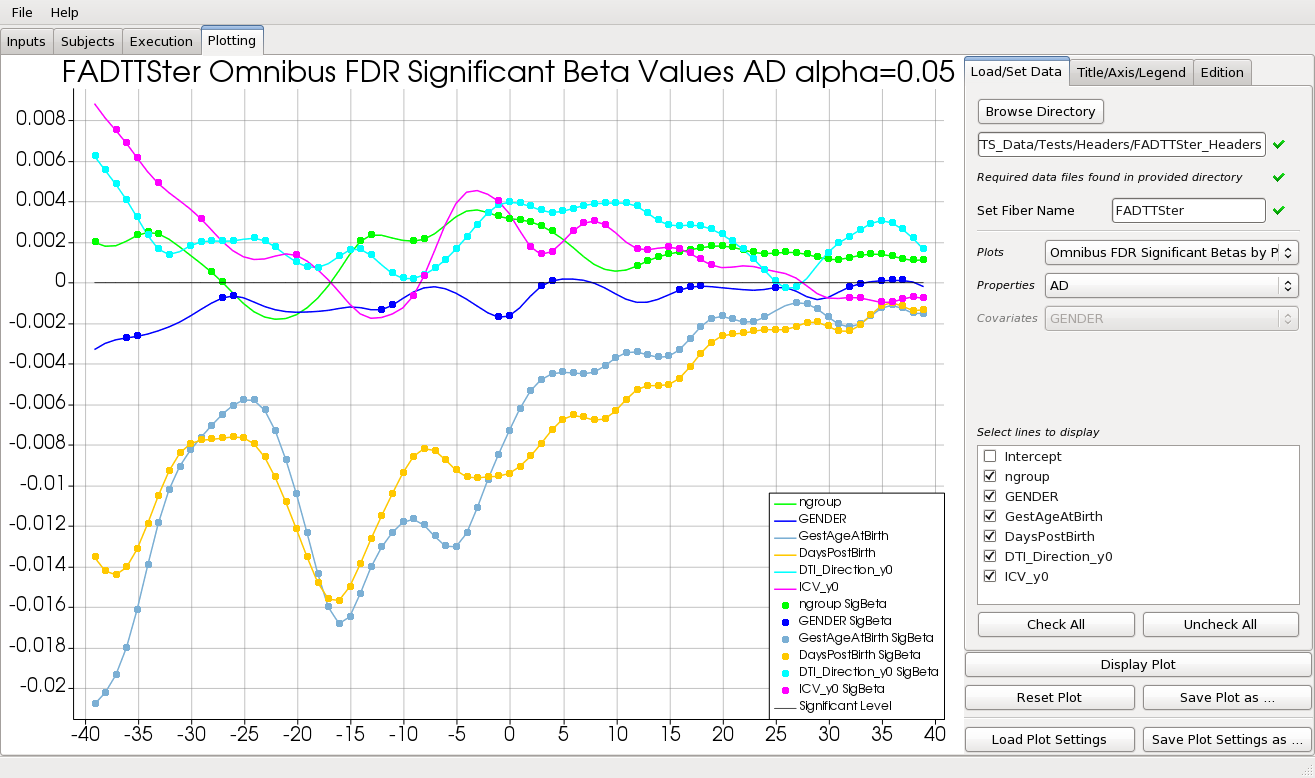
\includegraphics[width=0.95\textwidth,center]{omnibusFDRSigBetasProp}
  			\caption{Plotting omnibus FDR significant betas by properties}
    		\label{fig:omnibusFDRSigBetasProp}
		\end{figure}
		\item \textbf{Omnibus FDR Significant Betas by Covariates}\\
		Property\textrightarrow not required\\
		Covariate\textrightarrow mandatory
		\begin{figure}[H]
  			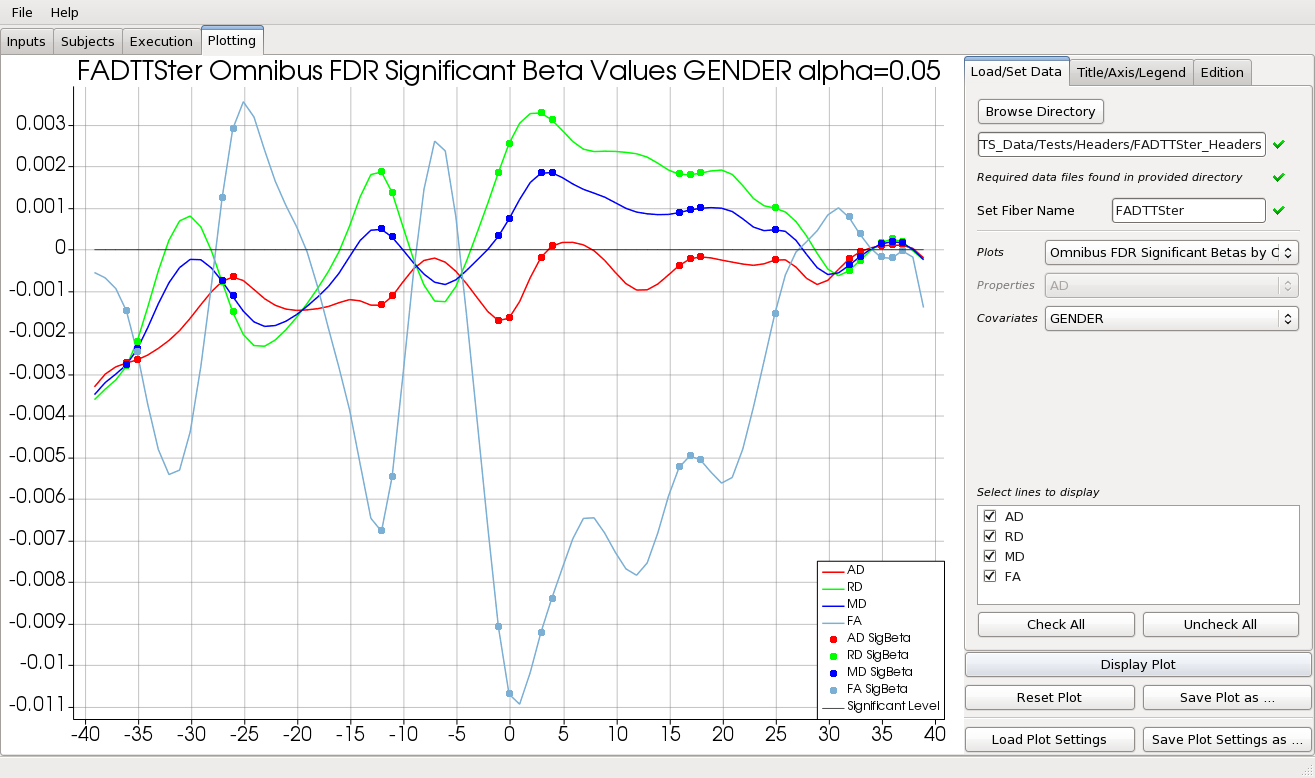
\includegraphics[width=0.95\textwidth,center]{omnibusFDRSigBetasCov}
  			\caption{Plotting omnibus FDR significant betas by covariates}
    		\label{fig:omnibusFDRSigBetasCov}
		\end{figure}
		\vfill
		\newpage
		
		\item \textbf{Omnibus Betas with Confidence Bands}\\
		Property\textrightarrow mandatory\\
		Covariate\textrightarrow optional
		\begin{figure}[H]
  			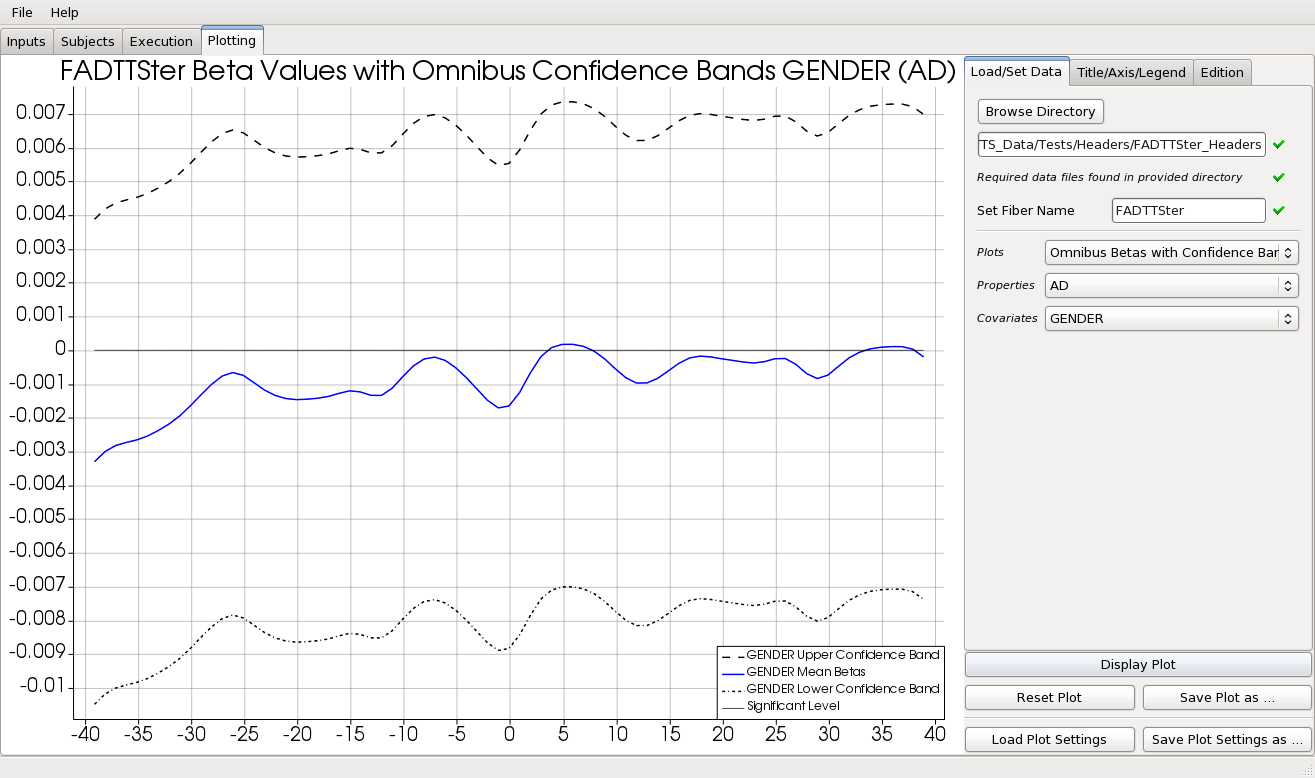
\includegraphics[width=0.95\textwidth,center]{omnibusBetasConfBands}
  			\caption{Plotting omnibus betas with confidence bands}
    		\label{fig:omnibusBetasConfBands}
		\end{figure}
		\item \textbf{Post-Hoc FDR Local pvalues by Covariates}\\
		Property\textrightarrow not required\\
		Covariate\textrightarrow mandatory
		\begin{figure}[H]
  			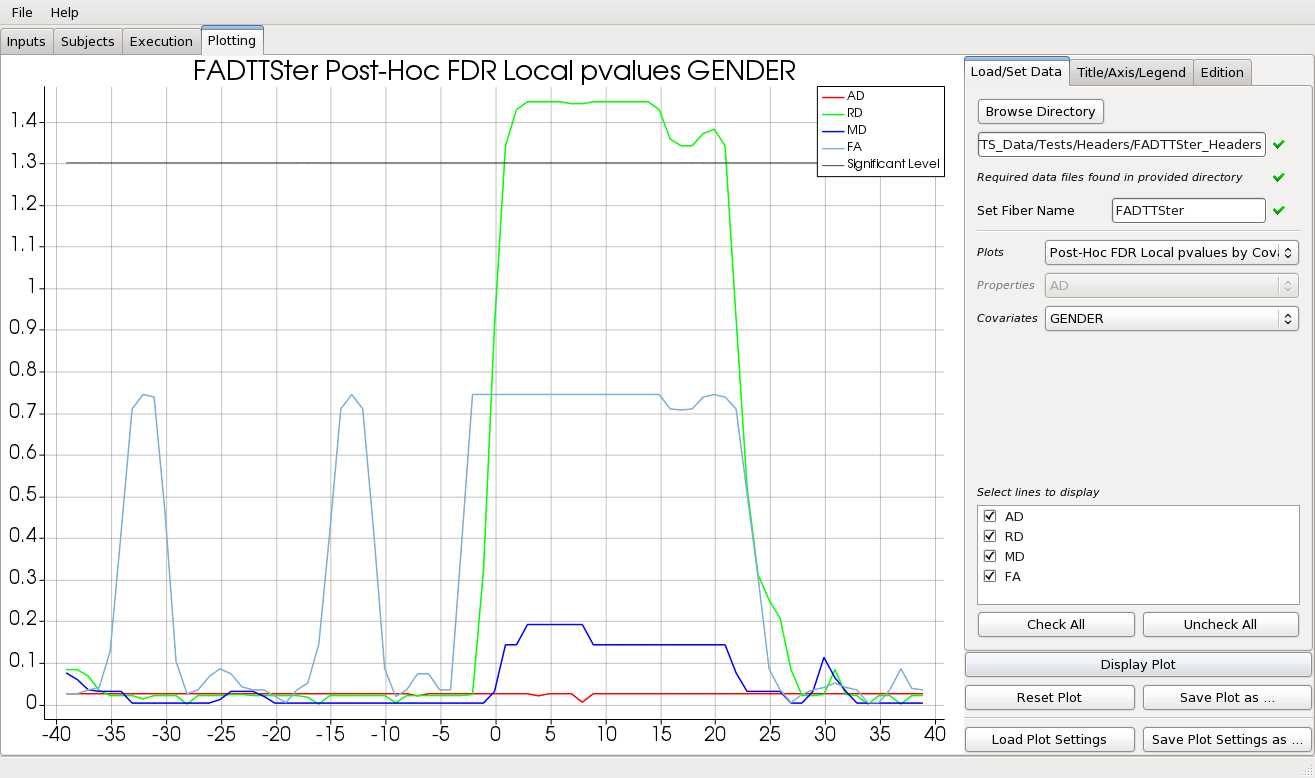
\includegraphics[width=0.95\textwidth,center]{phFDRLpCov}
  			\caption{Plotting post-hoc FDR local pvalues by covariates}
    		\label{fig:phFDRLpCov}
		\end{figure}
		\vfill
		\newpage
		
		\item \textbf{Post-Hoc FDR Significant Betas on Average Raw Data}\\
		Property\textrightarrow mandatory\\
		Covariate\textrightarrow optional
		\begin{figure}[H]
  			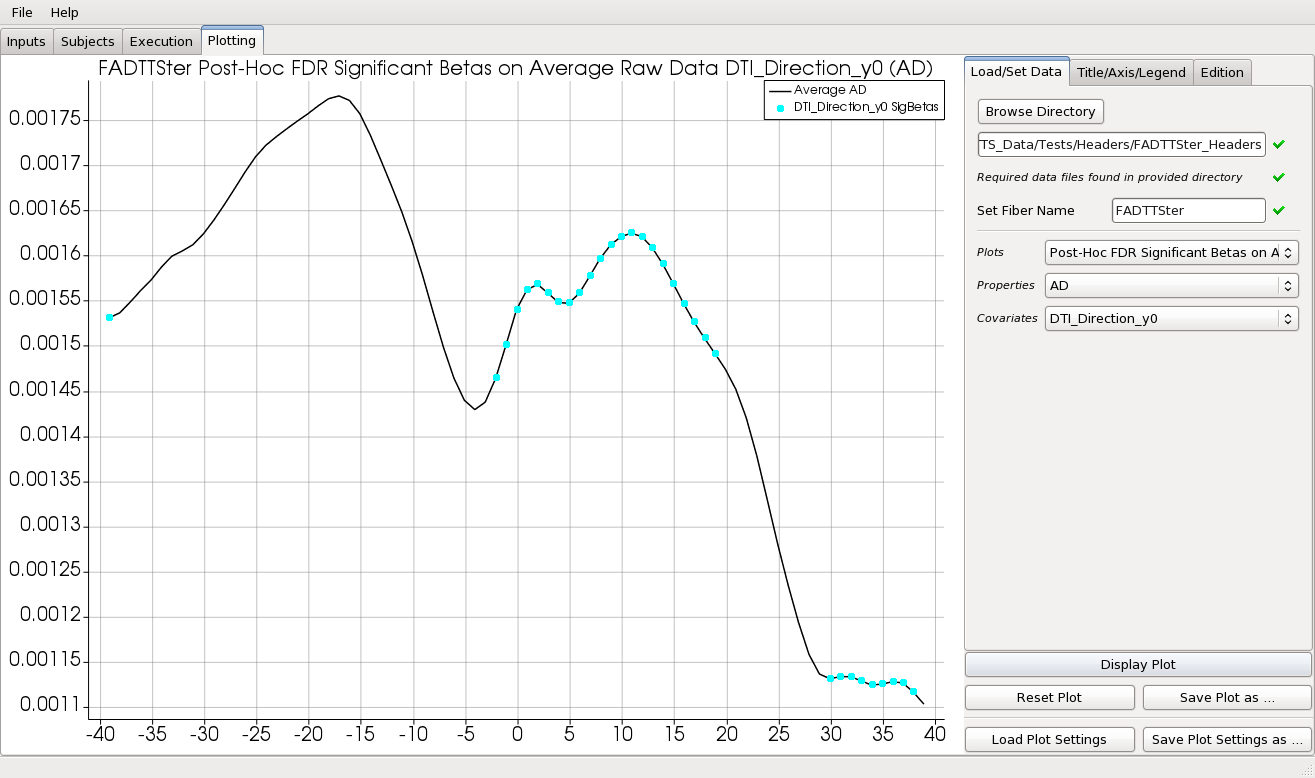
\includegraphics[width=0.95\textwidth,center]{phFDRSigBetasAvg1}
  			\caption{Plotting post-hoc FDR significant betas on average raw data}
    		\label{fig:phFDRSigBetasAvg1}
		\end{figure}
		\item \textbf{Post-Hoc FDR Significant Betas by Properties}\\
		Property\textrightarrow mandatory\\
		Covariate\textrightarrow not requiered
		\begin{figure}[H]
  			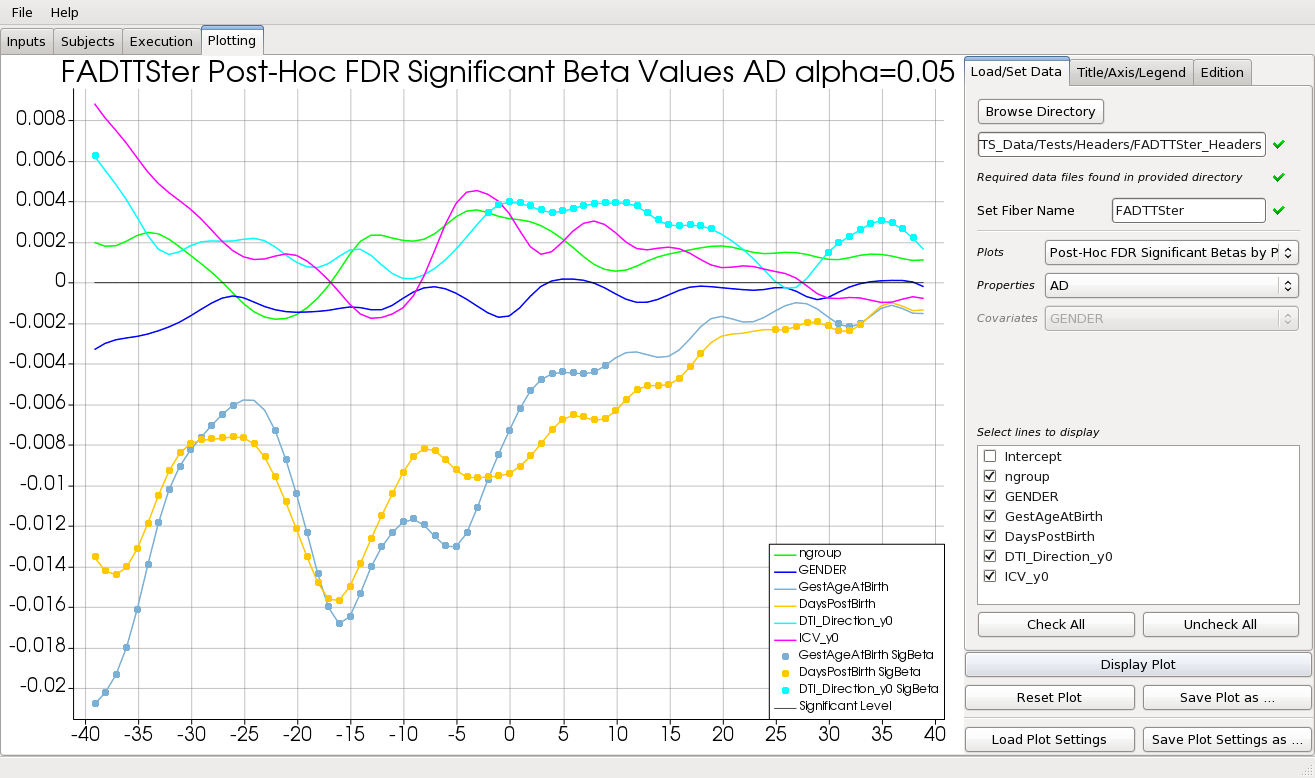
\includegraphics[width=0.95\textwidth,center]{phFDRSigBetasProp}
  			\caption{Plotting post-hoc FDR significant betas by properties}
    		\label{fig:phFDRSigBetasProp}
		\end{figure}
		\vfill
		\newpage
		
		\item \textbf{Post-Hoc FDR Significant Betas by Covariates}\\
		Property\textrightarrow not requiered\\
		Covariate\textrightarrow mandatory
		\begin{figure}[H]
  			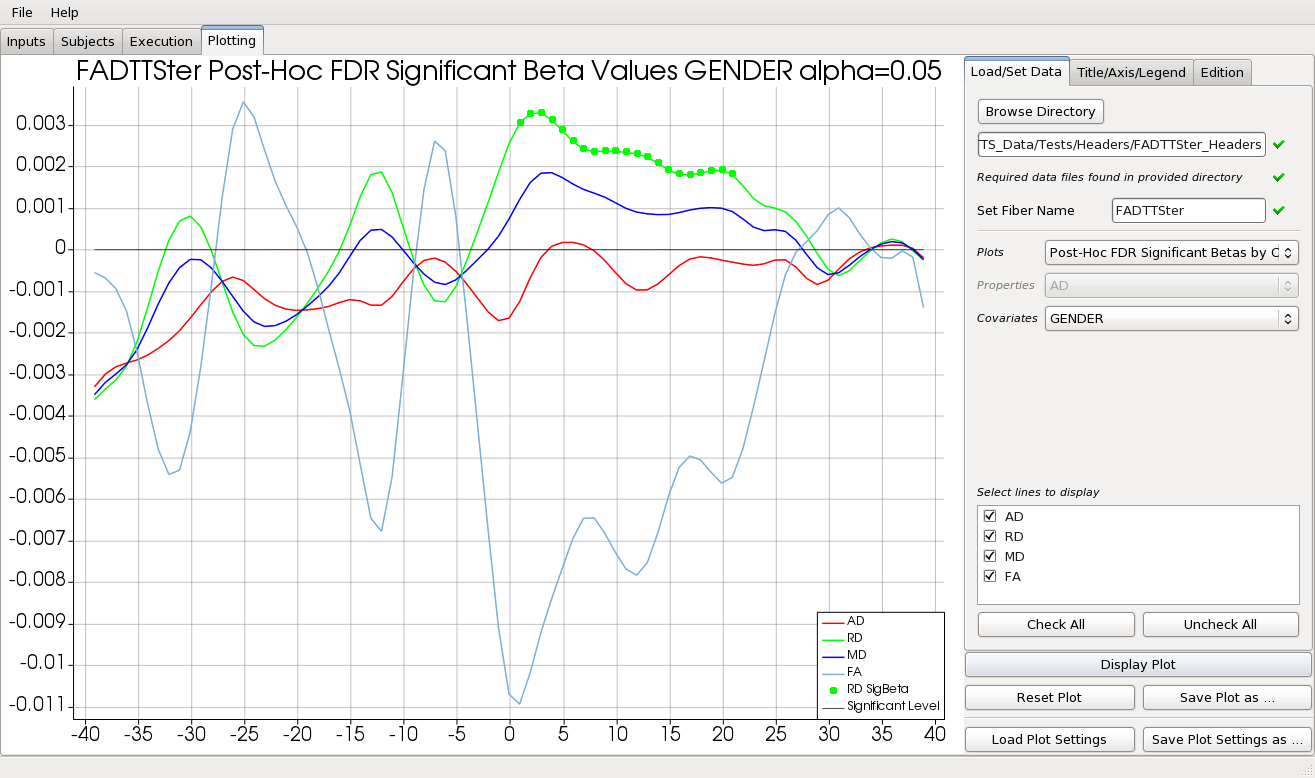
\includegraphics[width=1.1\textwidth,center]{phFDRSigBetasCov}
  			\caption{Plotting post-hoc FDR significant betas by covariates}
    		\label{fig:phFDRSigBetasCov}
		\end{figure}
	\end{itemize}
	\vfill
	\newpage	
	
	\subsection{Customize plot}
	To customize the plots and enhance the results, the user can use the features available in the tabs \textit{Title/Axis/Legend} and \textit{Edition}.
	\begin{figure}[H]
		\makebox[\linewidth][c]{
			\centering
			\begin{subfigure}{0.65\textwidth}
       			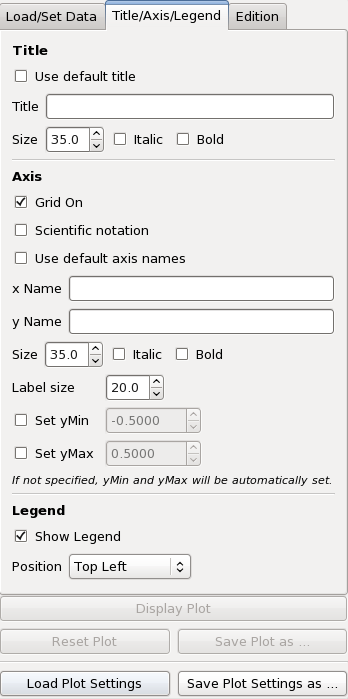
\includegraphics[width=\textwidth]{settings_blank1}
       			\caption{Title/Axis/Legend tab}
       			\label{subfig:settings_blank1}
    		\end{subfigure}
    		\begin{subfigure}{0.665\textwidth}
       			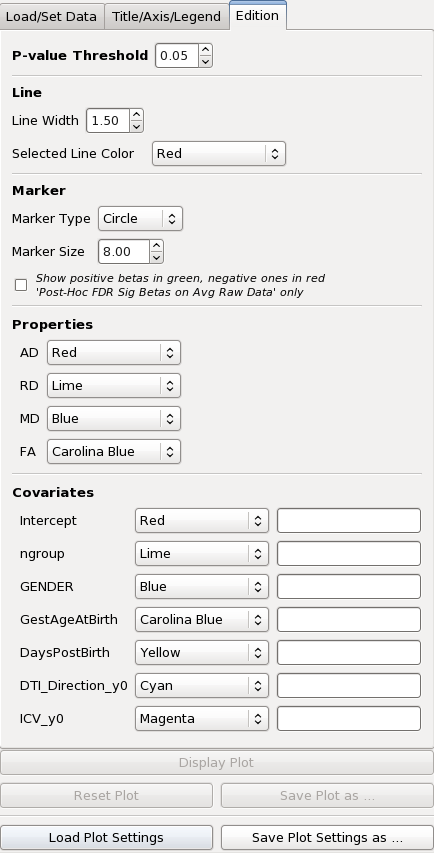
\includegraphics[width=\textwidth]{settings_blank2}
       			\caption{Edition tab}
       			\label{subfig:settings_blank2}
    		\end{subfigure}}
    	\caption{Plot customization tabs}
    	\label{fig:plotCustomization}
	\end{figure}	
	\vfill
	\newpage
	
	\subsubsection{Title/Axis/Legend Tab}
 	\begin{itemize}
 		\item \textbf{Title}
 		\begin{itemize}
 			\item \textit{Use default title:} If checked, the title is automatically generated based on the plot displayed and the fiber name
 			\item \textit{Title:} Sets the title displayed (used only if \textit{Use default title} is unchecked)
 			\item \textit{Size:} Sets the size of the title (value between 10 and 80)
 			\item \textit{Italic:} If checked, sets the title in italic
 			\item \textit{Bold:} If checked, makes the title bold
 		\end{itemize}
 		\item \textbf{Axis}
 		\begin{itemize}
 			\item \textit{Gird on:} Enables/disables the grid on the plotting area
 			\item \textit{Scientific notation:} Enables/disables the scientific notation for the axis
 			\item \textit{Use default axis names:} If checked, the axis names are automatically generated based on the plot displayed
 			\item \textit{x Names:} Sets the x axis name (used only if \textit{Use default axis names} is disabled)
 			\item \textit{y Names:} Sets the y axis name (used only if \textit{Use default axis names} is disabled)
 			\item \textit{Size:} Sets the size of the axis names (value between 10 and 80)
 			\item \textit{Italic:} If checked, sets the axis names in italic
 			\item \textit{Bold:} If checked, sets the axis names in bold
 			\item \textit{Label size:} Sets the size of the axis labels (value between 10 and 40)
 			\item \textit{Set yMin:} Enables/disables a minimum value for the y axis (value between -100 and 100)
 			\item \textit{Set yMax:} Enables/disables a maximum value for the y axis (value between -100 and 100)
 		\end{itemize}
 		\item \textbf{Legend}
 		\begin{itemize}
 			\item \textit{Show Legend:} Enables/disables the legend
 			\item \textit{Position:} Set the position of the legend on the plotting area\\
 			(\textit{Top Left/Top Center/Top Right/Middle Left/Middle Center/Middle Right/Bottom Left/Bottom Center/Bottom Right})
 		\end{itemize}
 	\end{itemize}
 	\vfill
	\newpage
	
	\begin{figure}[H]
  		\centering
    	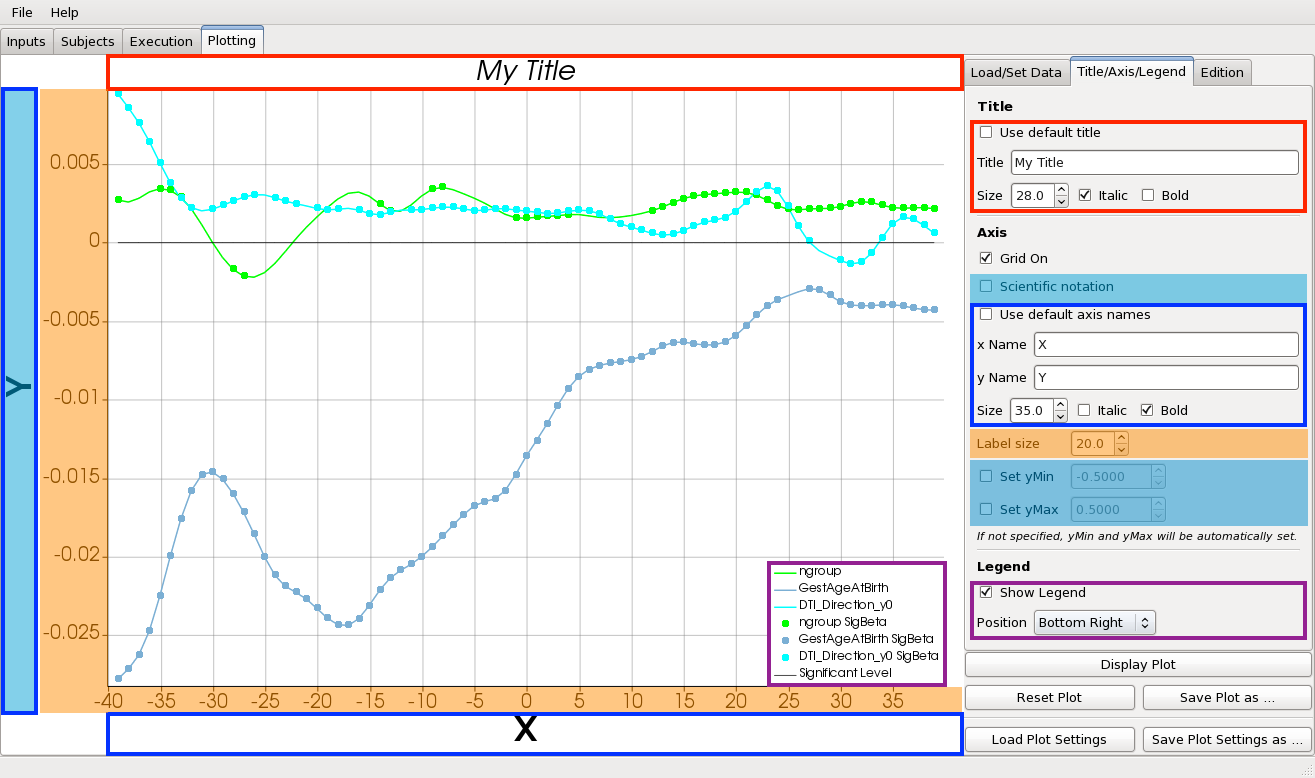
\includegraphics[angle=90,height=1.0\textheight]{settingsPlot}
    	\caption{Plot customization (1/2)}
    	\label{fig:settingsPlot}
    \end{figure}
    \vfill
	\newpage
	
	\subsubsection{Edition Tab}
	\begin{itemize}
		\item \textbf{P-value threshold}\\
		Sets the p-value threshold (value between 0 and 1)
		\item \textbf{Line}
		\begin{itemize}
 			\item \textit{Line Width:} Sets the line width (value between 0 and 1)
 			\item \textit{Color:} Sets the line color\\
 			(\textit{Red/Lime/Blue/Carolina Blue/ Yellow/Cyan/Magenta/Olive/Teal/Purple/Rosy Brown/Park Sea Green/ Corn Flower Blue/Maroon/Green/Navy/Orange/Mint/Pink/Brown/Black}) 
 		\end{itemize}
		\item \textbf{Marker}
		\begin{itemize}
 			\item \textit{Marker Type:} Sets the marker type\\
 			(\textit{Circle/Cross/Diamond/Plus/Square})
 			\item \textit{Color:} Sets the marker size (value between 4 and 20)
 			\item \textit{Show positive betas in green, negative ones in red:} This option is for \textit{Post-Hoc FDR Significant Betas on Average Raw Data}. When enabled, positive betas are displayed in green, and negative ones in red. When disabled all betas have the same color.
 		\end{itemize}
		\item \textbf{Properties}
		Colors are automatically set to each property loaded. The user can change them if needed.\\
 			(\textit{Red/Lime/Blue/Carolina Blue/ Yellow/Cyan/Magenta/Olive/Teal/Purple/Rosy Brown/Park Sea Green/ Corn Flower Blue/Maroon/Green/Navy/Orange/Mint/Pink/Brown/Black}) 
		\item \textbf{Covariates}
		\begin{itemize}
			\item Colors are automatically set to each covariate loaded. The user can change them if needed.\\
 			(\textit{Red/Lime/Blue/Carolina Blue/ Yellow/Cyan/Magenta/Olive/Teal/Purple/Rosy Brown/Park Sea Green/ Corn Flower Blue/Maroon/Green/Navy/Orange/Mint/Pink/Brown/Black}) 
			\item The label of each covariate is extracted from the data file. If the user needs a more explicit one, it can be changed by simply writing the new label in the blank space on the third column. When no new label is provided, the orginal label is kept. To apply such modifications, the user must click on ``Display Plot''.
		\end{itemize}
	\end{itemize}
	\vfill
	\newpage
	
	\begin{figure}[H]
  		\centering
    	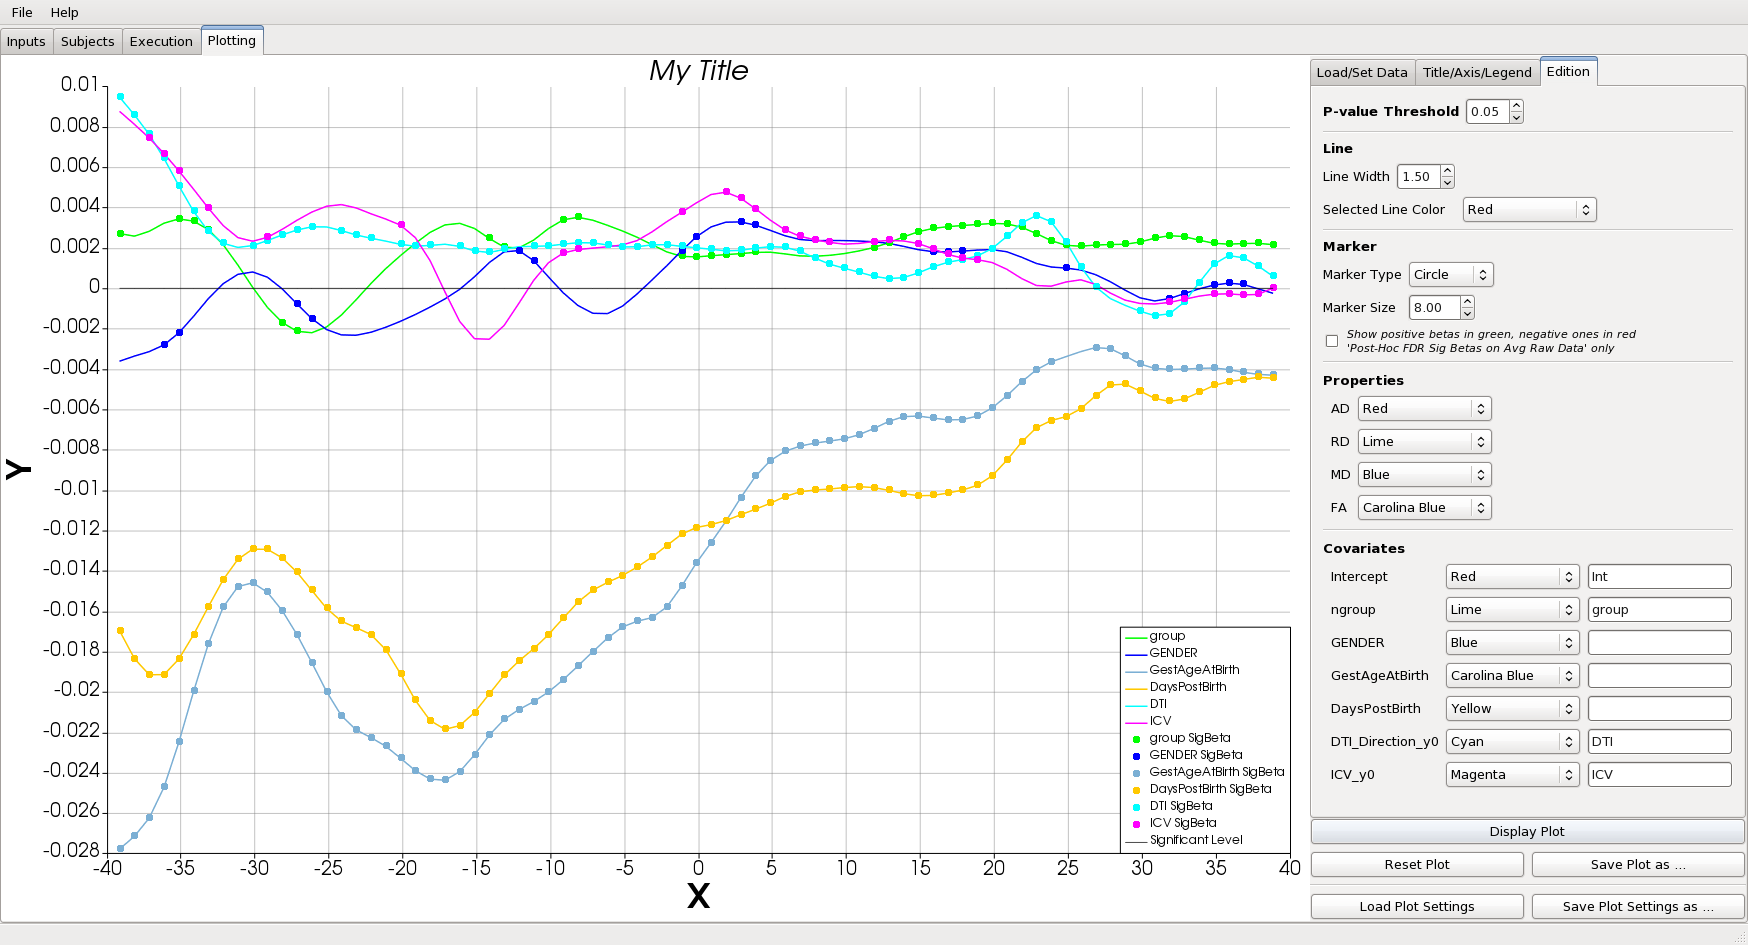
\includegraphics[angle=90,height=1.0\textheight]{settingsPlot_2}
    	\caption{Plot customization (2/2)}
    	\label{fig:settingsPlot_2}
    \end{figure}
    \vfill
	\newpage

	\subsubsection{Special Features}
	\begin{itemize}
		\item \textbf{Select Lines}\\
		When plotting the raw data, the user may select the lines displayed. If a line is selected, it is highlighted in red and the subject ID is displayed.
		\begin{figure}[H]
			\makebox[\linewidth][c]{
				\centering
				\begin{subfigure}{0.65\textwidth}
    	   			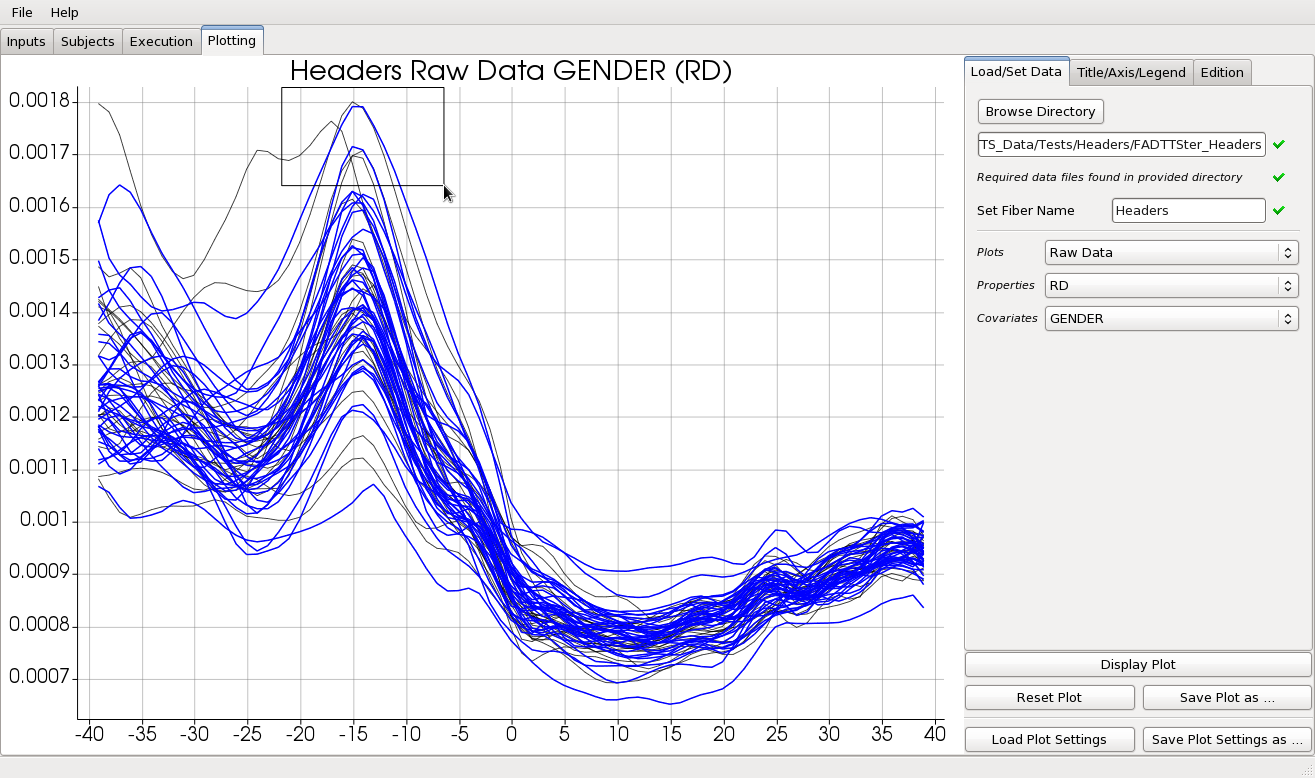
\includegraphics[width=\textwidth]{selectionPlot1}
       				\caption{Before}
       				\label{subfig:selectionPlot1}
		   		\end{subfigure}
    			\begin{subfigure}{0.65\textwidth}
       				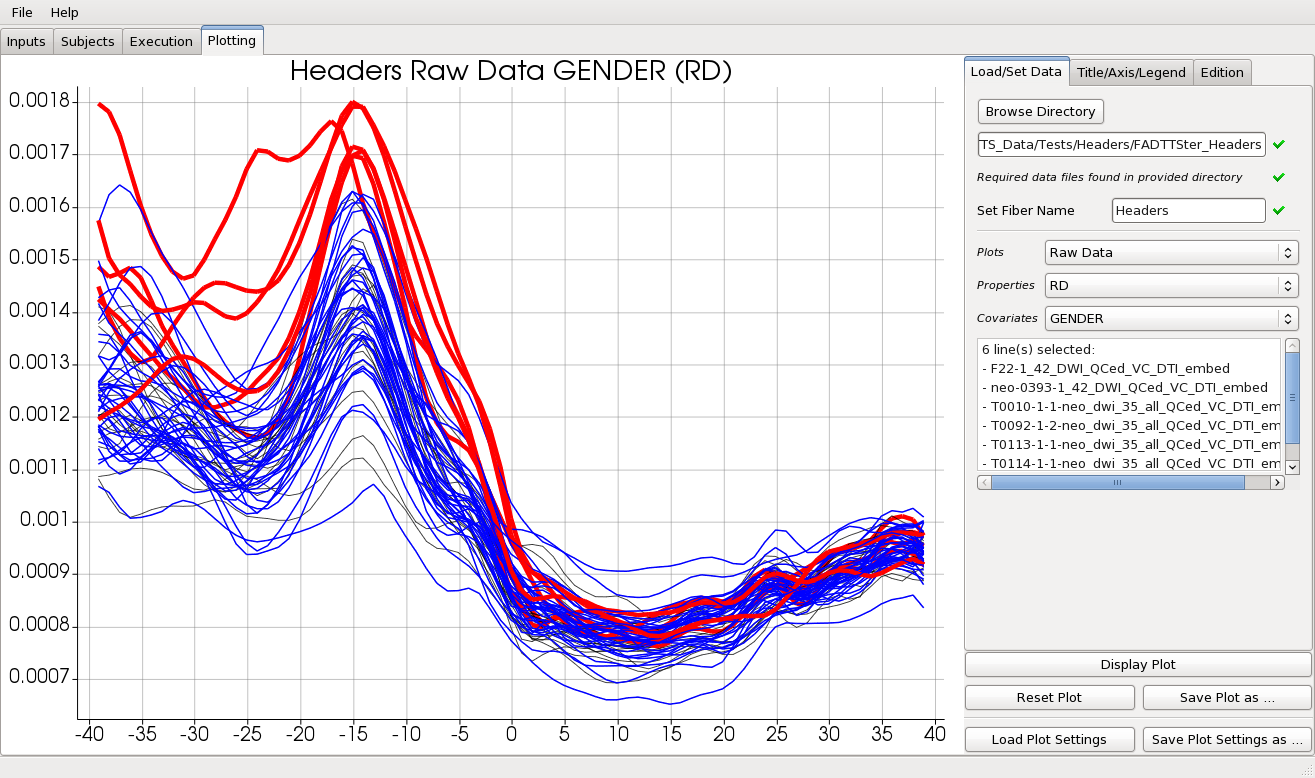
\includegraphics[width=\textwidth]{selectionPlot2}
       				\caption{After}
       				\label{subfig:selectionPlot2}
	 	   	\end{subfigure}}
    		\caption{Line selection when plotting raw data}
    		\label{fig:lineSelection}
		\end{figure}
		\item \textbf{Choose properties/covariates to display}\\
		Some plots give the option to choose the line to display. If this is the case, and if the user chooses to enable/disable some lines, the plotting area will automatically be updated.
		\begin{figure}[H]
			\makebox[\linewidth][c]{
				\centering
				\begin{subfigure}{0.65\textwidth}
    	   			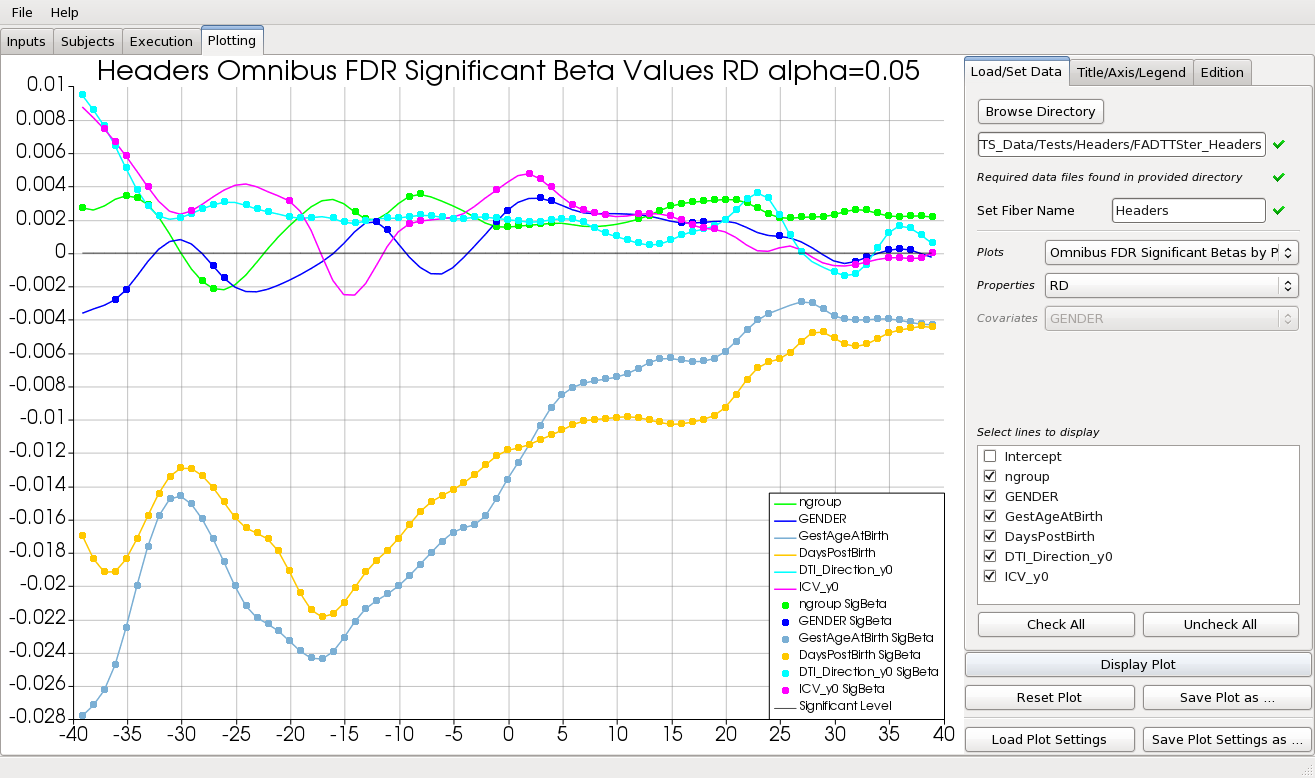
\includegraphics[width=\textwidth]{selectPropertiesPlot1}
       				\caption{Before}
       				\label{subfig:selectPropertiesPlot1}
		   		\end{subfigure}
    			\begin{subfigure}{0.65\textwidth}
       				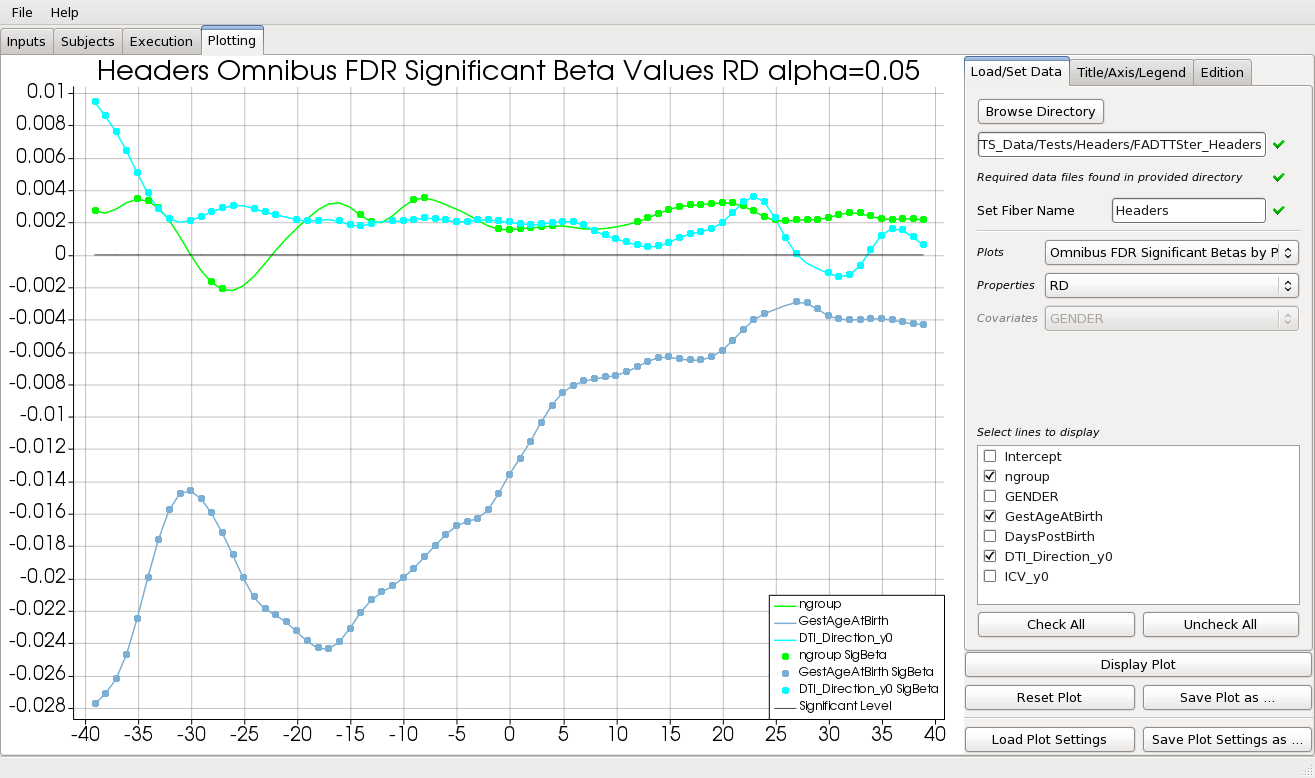
\includegraphics[width=\textwidth]{selectPropertiesPlot2}
       				\caption{After}
       				\label{subfig:selectPropertiesPlot2}
	 	   	\end{subfigure}}
    		\caption{For some plots, the user can choose the lines to display}
    		\label{fig:chooseLineToPlot}
		\end{figure}
	\end{itemize}
	\vfill
	\newpage
	
	\subsection{Save Plot}
	\begin{enumerate}
		\item Click on ``Save Plot as \ldots''
		\item In the pop-up window displayed, browse to the folder where you want to save your plot
		\item Rename the file if needed
		\item Click on ``Save''
	\end{enumerate}
	\subparagraph{\textbf{Note:}} File are saved as a .eps.
\end{document}